\chapter{Materiali}\label{chap:materiali}
Il cemento armato \`e un materiale composito formato dall'insieme di calcestruzzo e barre d'armatura in acciaio. Le caratteristiche meccaniche del composto saranno perci\`o funzione di entrambi i materiali.

Durante l'analisi e il progetto delle sezioni si utilizzeranno le seguenti ipotesi:
\begin{itemize}
    \item resistenza a trazione del calcestruzzo nulla agli SLU;
    \item perfetta aderenza tra acciaio e calcestruzzo;
    \item ipotesi di Bernoulli -- Navier per cui le sezioni ruotano, traslano e rimangono piane. Ne consegue che viene trascurata la deformabilit\`a a taglio degli elementi (ipotesi di elementi snelli).
\end{itemize}


\section{Calcestruzzo}
Il calcestruzzo utilizzato per il progetto \`e il $C25/30$ dove 
\begin{align}
	f_{ck} &= 25\,MPa, \label{eq:fck}\quad \text{resistenza di un provino cilindrico}\\
	R_{ck} &= 30\,MPa, \quad \text{resistenza di un provino cubico}
\end{align}

Secondo il capitolo \textbf{4.1.2.1.1.1 Resistenze di progetto a compressione del calcestruzzo} delle \ntc la resistenza in compressione $f_{cd}$ del calcestruzzo deve essere calcolata come
\[ 
f_{cd} = \dfrac{\alpha_{cc}\,f_{ck}}{\gamma_c}
\]
dove $\alpha_{cc}$ \`e un coefficiente riduttivo per gli effetti di lunga durata e vale $0.85$, $f_{ck}$ \`e la resistenza caratteristica definita sopra e $\gamma_c = 1.5$ \`e il coefficiente di sicurezza del materiale. La resistenza di progetto vale
\begin{equation}
	f_{cd} = \dfrac{0.85\cdot 25}{1.5} = 14.17\,MPa\label{eq:fcd}
\end{equation}

Il valore medio della resistenza cilindrica, utile per valutare il valore del modulo di Young medio del calcestuzzo, \`e definito -- secondo la \textbf{[11.2.2]} al punto \textbf{11.2.10.1} delle \ntc -- come segue
\[
f_{cm} = f_{ck} + 8\,MPa = 33\,MPa\\
\]

Causa variabilit\`a del modulo di elasticit\`a, il valore istantaneo va definito attraverso un modulo secante; ci\`o nonostante in fase di progettazione la normativa italiana consente l'utilizzo di un modulo di elasticit\`a medio definito come segue

\[
E_{cm} = 22000 \cdot \left(\dfrac{f_{cm}}{10}\right)^{0.3} = 22000\cdot\left(\dfrac{33}{10}\right)^{0.3} \simeq 31476\,MPa = 31.476\,GPa
\]

La resistenza di progetto a trazione del calcestruzzo \`e definita nel \textbf{4.1.2.1.1.2} delle \ntc come 
\[
f_{ctd} = \dfrac{f_{ctk}}{\gamma_c}
\]
dove $f_{ctk}$ \`e la resistenza caratteristica a trazione del calcestruzzo (\textbf{NTC 2018 -- 11.2.10.2})
\begin{align}
	f_{ctm} &= 0.30\cdot f_{ck}^{2/_3} = 0.30\cdot 25^{2/_3}\,MPa = 2.57\,MPa\label{eq:fctm}\\
	f_{ctk,0.05} &= 0.7\cdot f_{ctm} = 0.7\cdot 2.57\,MPa = 1.80\,MPa\label{eq:fctk005}
\end{align}
che risulta coincidente con la \textbf{Table 3.1 -- EC2}. La resistenza di progetto a trazione \`e perci\`o
\begin{equation}
	\label{eq:fctd}
	f_{ctd} = \alpha_{ct}\,\dfrac{f_{ctk,0.05}}{\gamma_c} = 0.85\,\dfrac{1.8}{1.5} = 1.02\,MPa
\end{equation}

L'\ec, al punto \textbf{} definisce la tensione tangenziale di aderenza tra acciaio e calcestruzzo, che sar\`a necessaria durante il calcolo delle lunghezze di ancoraggio delle barre. Secondo le definizioni \textit{(8.2)} la tensione di ancoraggio di progetto è
\begin{equation}
	\label{eq:fbd}
	f_{bd} = 2.25\cdot\eta_1\,\eta_2\,f_{ctd}
\end{equation}
dove $\eta_1$ dipende dalle condizioni di aderenza (buona o non buona) e $\eta_2$ dipende dal diametro delle barre di armatura.

Infine, in prima approssimazione, si sceglie un diametro massimo degli inerti pari a
\[
    d_g = 20\,mm
\]

\subsection{Legame costitutivo del calcestruzzo}

\begin{figure}
    \centering
	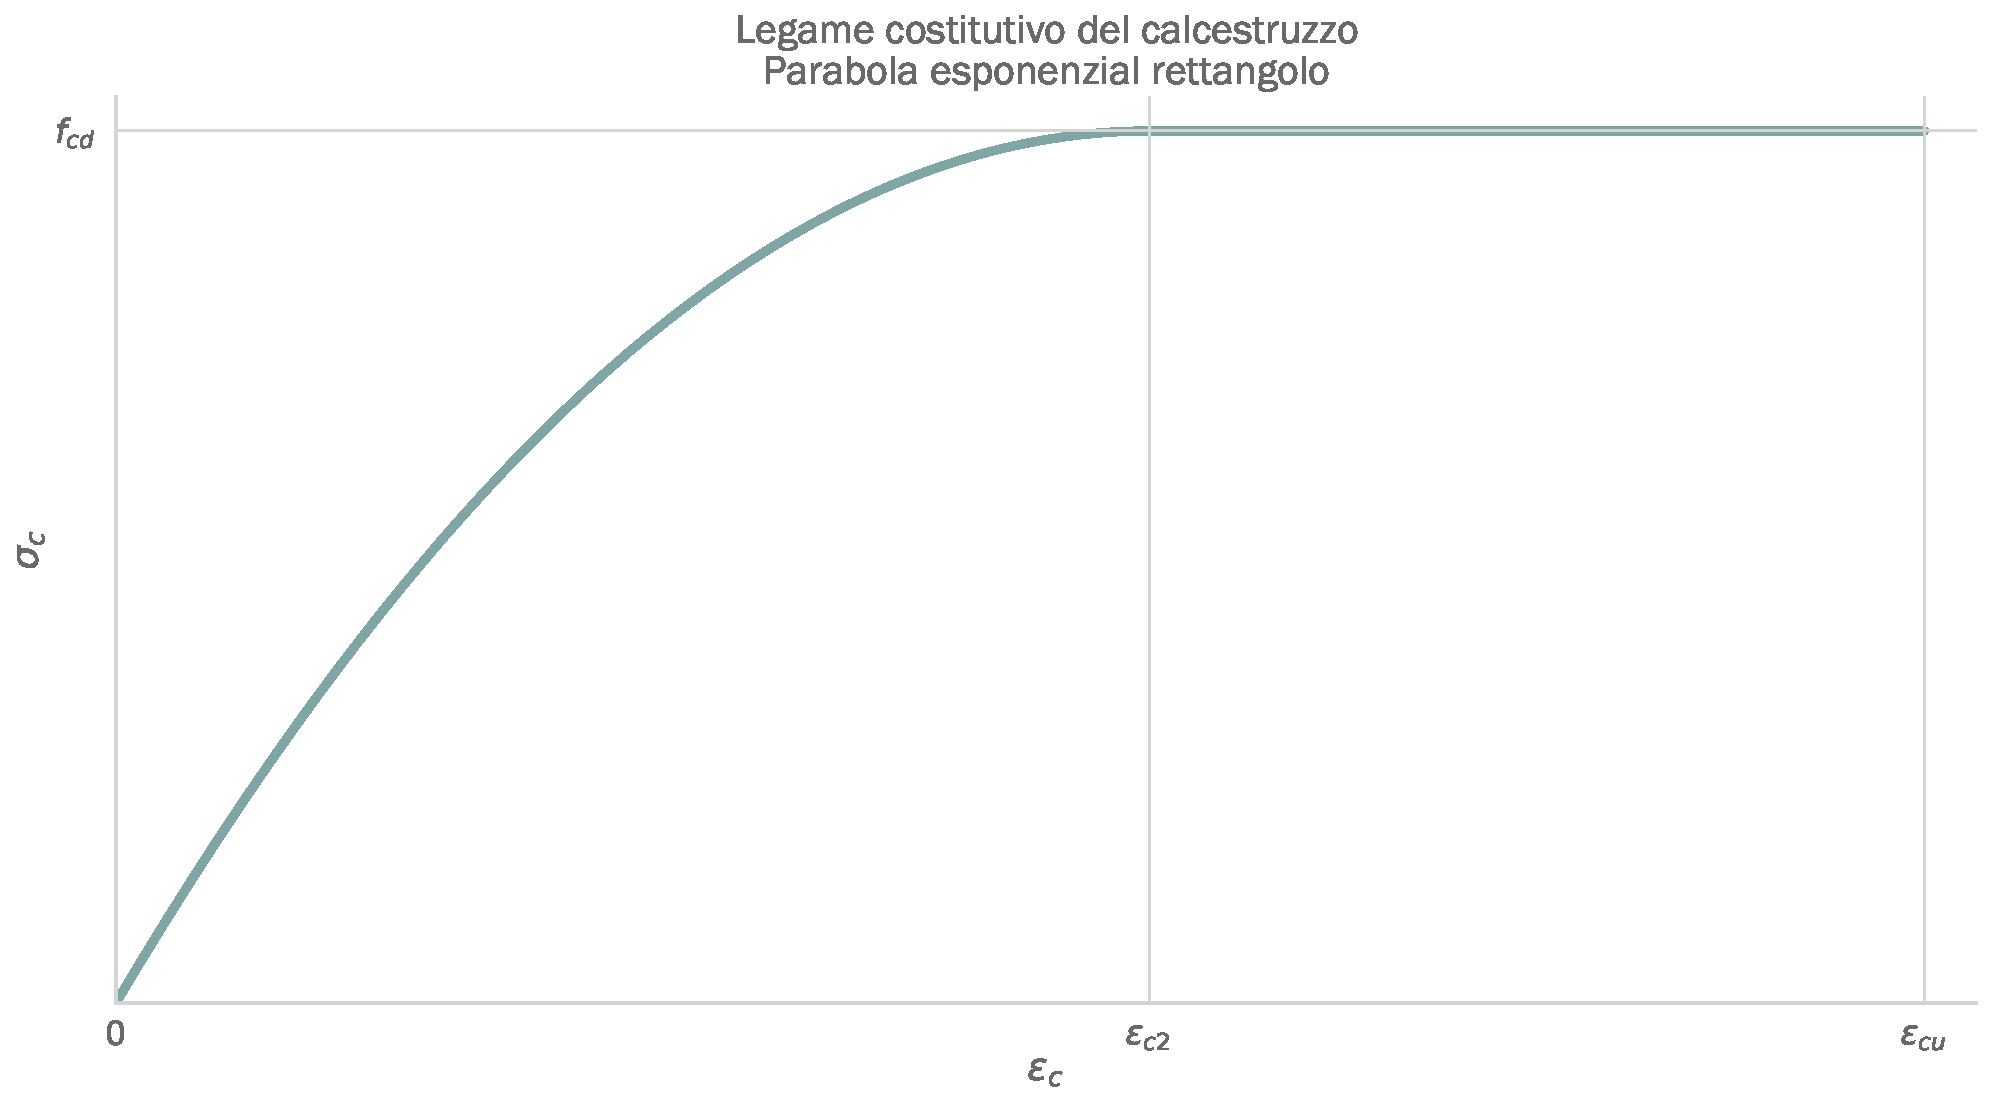
\includegraphics[width=\textwidth]{legameCostitutivoCLS}
	\caption{Legame costitutivo parabola esponenzial rettangolo}
	\label{fig:legameCostitutivoCLS}
\end{figure}

\begin{figure}
	\centering
	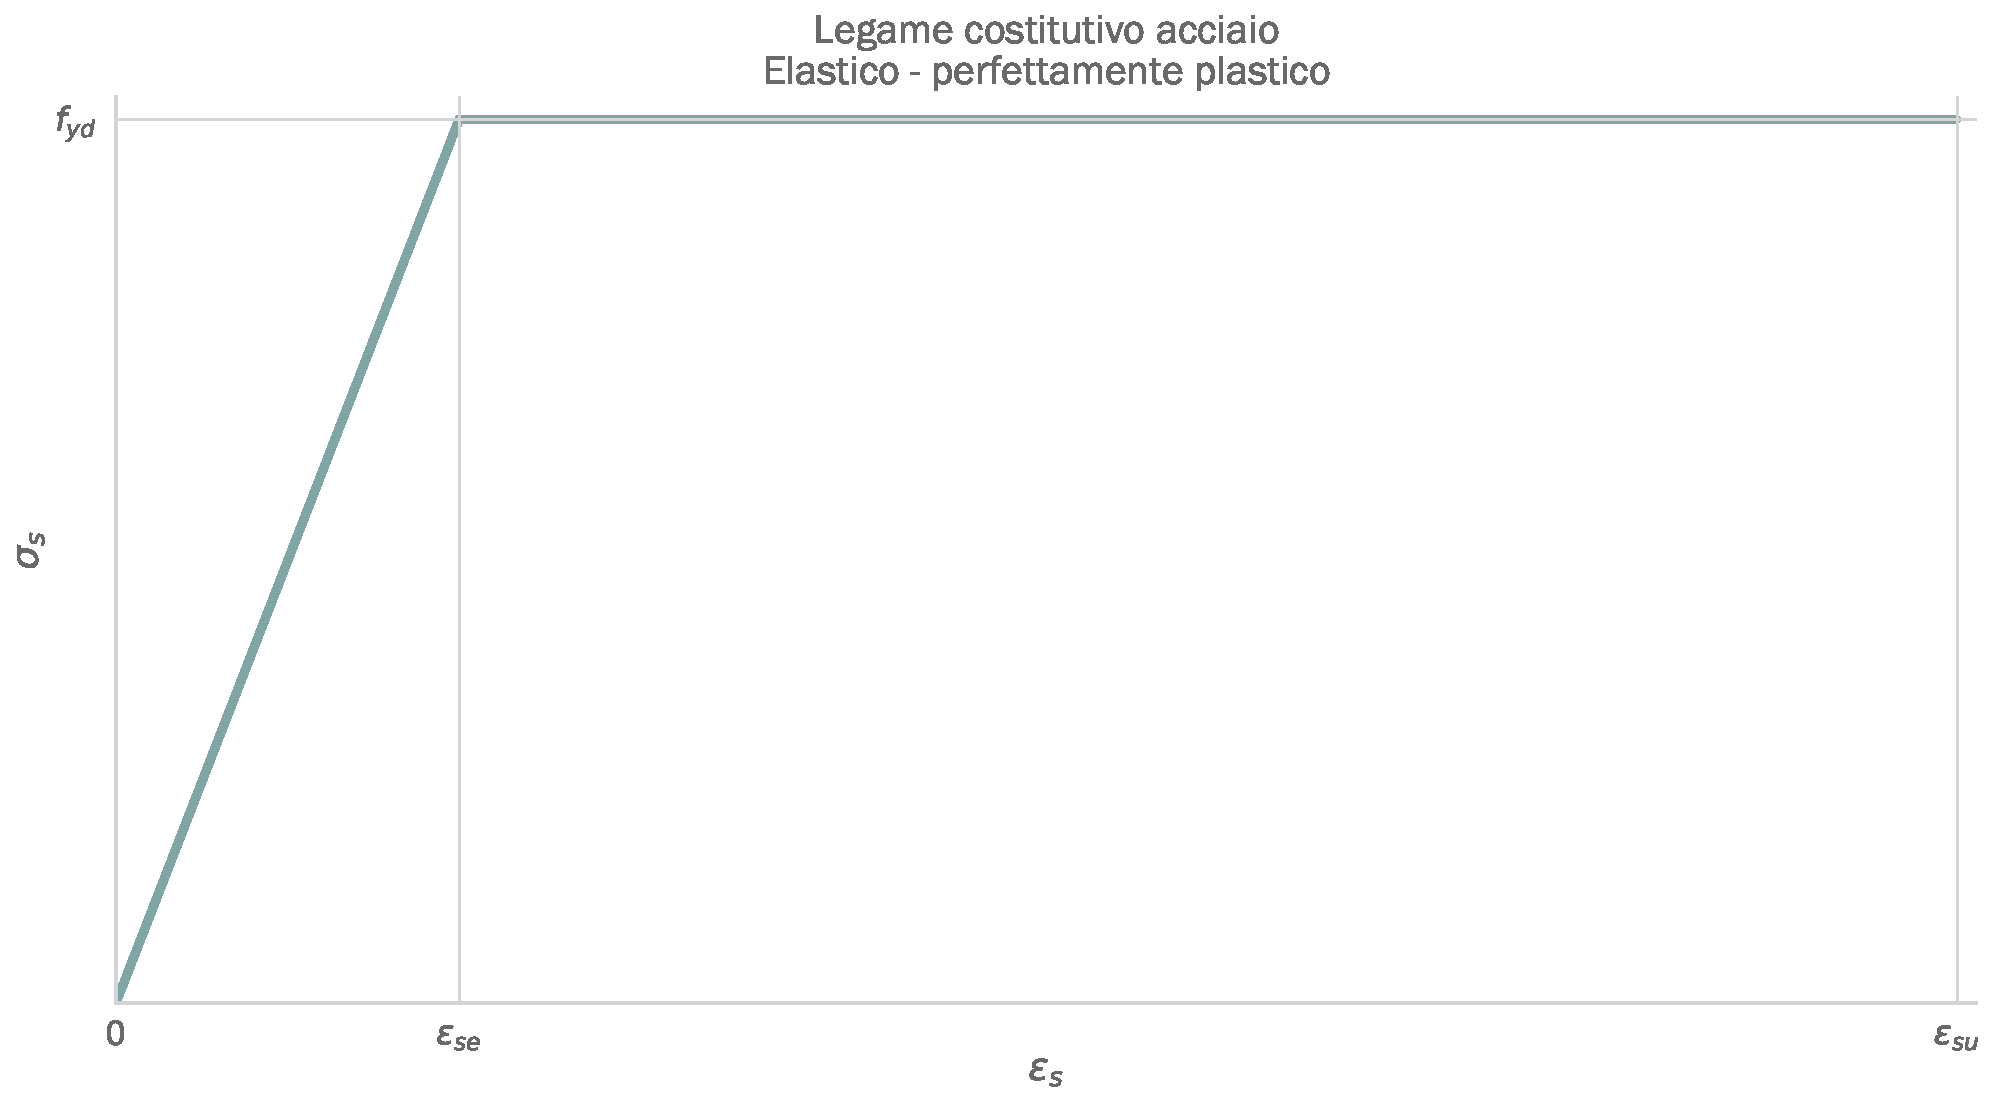
\includegraphics[width=\textwidth]{legameCostitutivoAcciaio}
	\caption{Legame costitutivo elastico -- perfettamente plastico}
	\label{fig:legameCostitutivoAcciaio}
\end{figure}

Il legame costitutivo tensione--deformazione del calcestruzzo scelto per il progetto e la verifica agli SLU di tutti gli elementi in esame \`e il \emph{parabola esponenzial rettangolo}, definito al punto \textbf{4.1.2.1.2.1} delle \ntc o in alternativa al punto \textbf{3.1.7} del \textbf{EC2}. L'equazione che descrive le curva \`e la seguente
\begin{equation}
	\sigma_c = \begin{cases}
		f_{cd}\,\left[1-\left(1-\dfrac{\epsilon_c}{\epsilon_{c2}}\right)^n\,\right],\qquad &\epsilon_c \in [0, \epsilon_{c2}]\\
		f_{cd} &\epsilon_c > \epsilon_{c2}
	           \end{cases}
	\label{eq:legameCostitutivoCLS}
\end{equation}
dove $n=2$ per calcestruzzi di classe minore o tuttalpi\`u uguale alla $C50/60$. Il diagramma \`e quello rappresentato in figura~\ref{fig:legameCostitutivoCLS}. I valori di $\epsilon_{c2}$ e $\epsilon_{cu}$ dipendono anch'essi dalla classe del calcestruzzo. In particolare, per classi pari o inferiori alla $C50/60$
\begin{align*}
	\epsilon_{c2} &= 2\permil\\
	\epsilon_{cu} &= 3.5\permil
\end{align*}

Come accennato sopra, durante il progetto e la verifica agli SLU, verr\`a considerata nulla la resistenza a trazione del calcestruzzo; al contrario, durante le verifiche di deformazione e fessurazione agli SLE si vede la necessit\`a di introdurre la resistenza a trazione del calcestruzzo, definita nelle \eqref{eq:fctm}, \eqref{eq:fctk005} e \eqref{eq:fctd}.

\section{Acciaio}
La normativa italiana al punto \textbf{11.3.2} ammette un unico acciaio per armatura: \textbf{B450C}. Questo acciaio \`e caratterizzato dall'avere una tensione di snervamento caratteristica 
\[
f_{yk} = 450\,MPa
\]

La resistenza di progetto \`e valutata come
\begin{equation}
    \label{eq:fyd}
	f_{yd} = \dfrac{f_{yk}}{\gamma_s} = \dfrac{450}{1.15} = 391.30\,MPa
\end{equation}
dove il coefficiente di sicurezza per l'acciaio d'armatura vale $\gamma_s = 1.15$.

Si assume inoltre un modulo di elasticit\`a pari a 
\begin{equation}
    \label{eq:Es}
	E_s = 210\cdot 10^3 MPa = 210\,GPa
\end{equation}

\`E quindi banale calcolare la deformazione al limite elastico, cio\`e la deformazione per cui avviene lo snervamento dell'acciaio
\begin{equation}
	\epsilon_{se} = \dfrac{f_{yd}}{E_s} = \dfrac{391.30}{210\cdot 10^3} = 1.863\permil
\end{equation}



\subsection{Legame costitutivo dell'acciaio}

Il legame tensione -- deformazione scelto per l'acciaio \`e quello di \emph{elastico -- perfettamente plastico}, con una deformazione massima a rottura limitata a 
\[
\epsilon_{su} = 10\permil
\]

Fissare un limite alla deformazione a rottura non \`e un'imposizione della normativa ma una comodit\`a in fase di progettazione delle sezioni.

\cleardoublepage
